\chapter{\uppercase{Research Directions} \label{chapter:05}}

Summary of NSF project, some OED stuff perhaps, functional assimilation.

\section{Sequential Inversion}\label{sec:ch05-sequential}

The DCI framework relies on evaluating the ration function $r(\param)$ in $\dimD$--dimensional QoI space, so we turn our attention to addressing the challenges associated with the growth of this space.
As $\dimD$ increases, we must approximate a push-forward distribution with perhaps a fixed number of samples (from model evaluations) $\nsamps$, which represents a considerable source of error since the convergence rate for kernel density estimation with Gaussian kernels is $\mathcal{O} (N^{2+\dimD})$.

For example, suppose we have a time-dependent problem for which hundreds of spatial sensors are providing streams of data.
Approximating a hundred-dimensional space with $\nsamps = 1E3$ or $1E4$ samples (as we have been using for demonstrations), is wrought with problems.
However, either of these values for $\nsamps$ would be sufficient to estimate a one-dimensional distribution.
In some sense, approximating a QoI at each location over time is reasonable, but doing so for all of them simultaneously is not.
To this end, we propose to investigate an approach to solving the parameter estimation problem by performing inversion through a sequence of scalar-valued QoIs rather than employ a vector-valued approach.

We could choose any dimension below $\dimD$, but this sequential-scalar-valued approach provides a starting place and admits a simplicity in exposition.
By choosing a dimension of 1, we can focus solely on the order in which QoIs are inverted and dismiss the additional complexity of enumerating the combinations of QoI when dimensions can vary.
We also choose to use a linear map for convenience so that we can use the analytical solutions presented in the previous chapter without concern for approximation error.

With each iteration in the sequence of inverse problems, we are in-effect trying to explain measurements that constitute a single QoI at the expense of accuracy in others.
By contrast, the vector-valued approach seeks accuracy in all of the simultaneously.
This tradeoff is all about convenience, since 1-dimensional problems are computationally ``cheap,'' we can iterate through many more of them for the same computational cost.
Since by the time we finish iterating through all available QoI, the error in $Q^{(1)}$ may have been allowed to drift quite significantly away from its solution contour through the sequence of inverting through $Q^{(1)}, Q^{(2)}, \dots Q^{(100)}$.
To address this, we perform multiple passes through our set of QoI.
Borrowing from other sequential algorithms, these ``epochs'' will allow us to iterate until the solution stops changing by some predefined relative threshold, representing a lack of ``learning'' through continued effort.

We study the following motivating two-dimensional example with QoI defined by ten equispaced rotations of the unit vector $[0, 1]$ through the first two Euclidean quadrants.
We first plot the result of a single epoch in Fig.~\ref{fig:iterative-linear-demo}
\begin{figure}
  \centering
  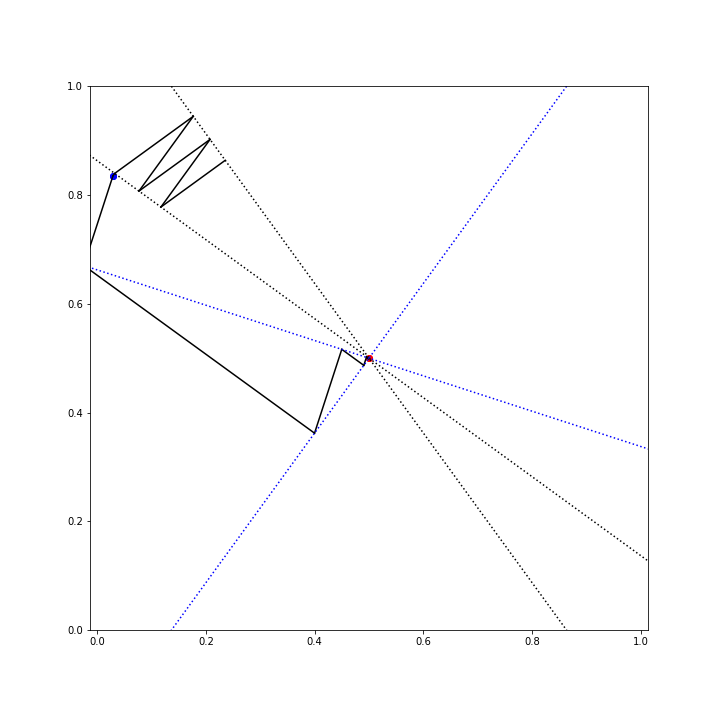
\includegraphics[width=0.475\linewidth]{examples/iterative/10D-firstepoch}
  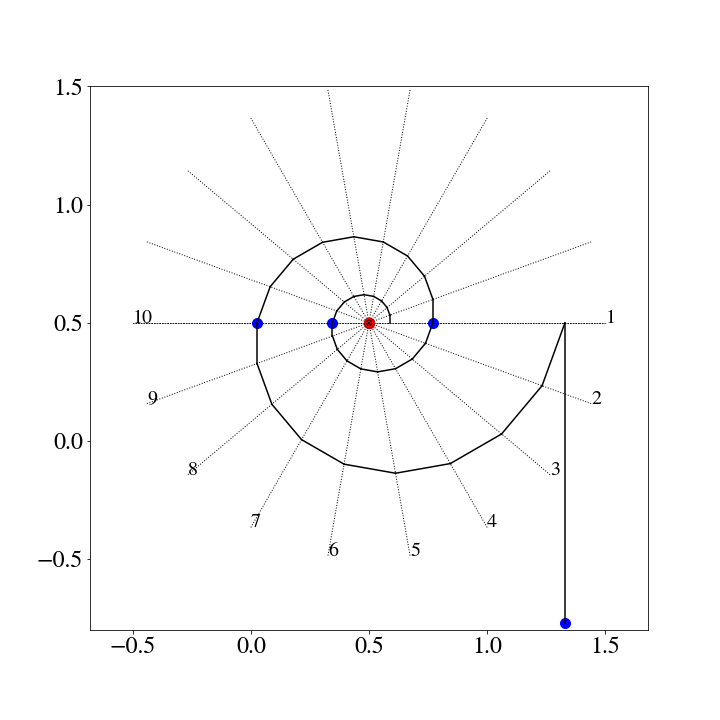
\includegraphics[width=0.475\linewidth]{examples/iterative/10D-fewepochs}

  \caption{
  Dotted lines show the solution contours for each row of the operator $A$.
  (Left): First epoch for iterating through 10 QoI.
  (Right): Three more epochs allows our estimate to get much closer to the true value.
  }
  \label{fig:iterative-linear-demo}
\end{figure}
\FloatBarrier

The spiral shape is a result of the underlying geometry of this QoI map defined by rotations. The successive rows are so similar to each other that very little is ``learned'' between each iteration; the projection doesn't cover a large distance in $\pspace$.
Contrast this to two random choices of a pair of indices among the ten, shown in Fig.~\ref{fig:iterative-linear-demo-pair}.

\begin{figure}
  \centering
  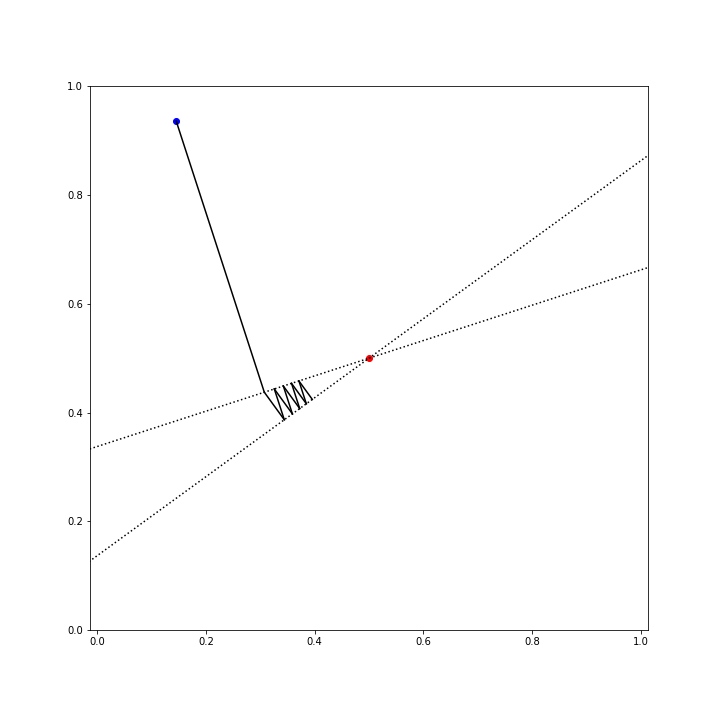
\includegraphics[width=0.475\linewidth]{examples/iterative/10D-fewepochs-pair}

  \caption{
  Dotted lines show the solution contours for each row of the operator $A$.
  (Left): First epoch for iterating through 10 QoI.
  (Right): Three more epochs allows our estimate to get much closer to the true value.
  }
  \label{fig:iterative-linear-demo-pair}
\end{figure}
\FloatBarrier


\section{Addressing Model Assumptions}\label{sec:ch05-variance}

What if we don't know the variance? How does mis-estimating it affect our solutions?

Multiplicative noise - handled in a straightforward way, maybe put an example here and leave it at that? Put it in appendix?


\section{Leveraging Data in Different Ways}\label{sec:ch05-data}

This section is effectively addressing how to use more data in different ways.

Would be nice to see a data-driven map done with the set-based framework first as an example.
May be appropriate in example for Ch 4.

\section{Optimal Experimental Design}\label{sec:ch05-oed}

Algorithm for sequentially choosing QoI, brief discussion of trade-offs of accuracy/precision.

\section{Machine-Learning Enhancements}\label{sec:ch05-ml}

how can we automate this process? Some mixture of sequential (how can we incorporate a new data point? start over? re-solve the problem? what's the cost?) approximations, maybe switching between the two approaches (set-based to reduce the parameter space, use that as the new initial).
